%%%%%%%%%%%%%%%%%%%%%%%%%%%%%%%%%%%%%%%%%%%%%%%%%%%%%%%%
%                IAML 2020 Assignment 1                %
%                                                      %
%                                                      %
% Authors: Oisin Mac Aodha and Octave Mariotti         %
% Using template from: Michael P. J. Camilleri and     %
% Traiko Dinev.                                        %
%                                                      %
% Based on the Cleese Assignment Template for Students %
% from http://www.LaTeXTemplates.com.                  %
%                                                      %
% Original Author: Vel (vel@LaTeXTemplates.com)        %
%                                                      %
% License:                                             %
% CC BY-NC-SA 3.0                                      %
% (http://creativecommons.org/licenses/by-nc-sa/3.0/)  %
%                                                      %
%%%%%%%%%%%%%%%%%%%%%%%%%%%%%%%%%%%%%%%%%%%%%%%%%%%%%%%%

%--------------------------------------------------------
%   IMPORTANT: Do not touch anything in this part
\documentclass[12pt]{article}
\input{style.tex}



% Options for Formatting Output

\global\setbool{clearon}{true} %
\global\setbool{authoron}{true} %



\newcommand{\assignmentQuestionName}{Question}
\newcommand{\assignmentTitle}{Assignment\ \#1}

\newcommand{\assignmentClass}{IAML -- INFR10069 (LEVEL 10)}

\newcommand{\assignmentWarning}{NO LATE SUBMISSIONS} % 
\newcommand{\assignmentDueDate}{Tues,\ October\ 20,\ 2020 @ 16:00}
%--------------------------------------------------------


%%%%%%%%%%%%%%%%%%%%%%%%%%%%%%%%%%%%%%%%%%%%%%%%%%%%%%%
%
% NOTE: YOU NEED TO ENTER YOUR STUDENT ID BELOW.
%
%%%%%%%%%%%%%%%%%%%%%%%%%%%%%%%%%%%%%%%%%%%%%%%%%%%%%%%%
%--------------------------------------------------------
% IMPORTANT: Specify your Student ID below. You will need to uncomment the line, else compilation will fail. Make sure to specify your student ID correctly, otherwise we may not be able to identify your work and you will be marked as missing.
\newcommand{\assignmentAuthorName}{s1864480}
%--------------------------------------------------------



\begin{document}
\maketitle
\thispagestyle{empty}







%%%%%%%%%%%%%%%%%%%%%%%%%%%%%%%%%%%%%%%%%%%%%%%%%%%%%%%%%%%%%%%%%%%%%%%%%%%%%%
%============================================================================%
%%%%%%%%%%%%%%%%%%%%%%%%%%%%%%%%%%%%%%%%%%%%%%%%%%%%%%%%%%%%%%%%%%%%%%%%%%%%%%
\clearpage

\begin{question}{(22 total points) Linear Regression}

\questiontext{In this question we will fit linear regression models to data.}



%
%
\begin{subquestion}{(3 points) Describe the main properties of the data, focusing on the size, data ranges, and data types.   
}


\begin{answerbox}{10em}
There are $50$ observations in the dataset. The observations have two attributes, \textit{revision\_time} and \textit{exam\_score} and both these attributes are of type \textit{float64}. We observe that revision time ranges from a minimum of $2.723$ hrs to maximum of $48.011$ hrs, and the exam scores ranges from $14.731$ to $94.945$.
\end{answerbox}



\end{subquestion}




%
%
\begin{subquestion}{(3 points) Fit a linear model to the data so that we can predict \texttt{exam\_score} from \texttt{revision\_time}. 
Report the estimated model parameters $\mathbf{w}$. 
Describe what the parameters represent for this 1D data. 
For this part, you should use the sklearn implementation of \href{https://scikit-learn.org/0.19/modules/generated/sklearn.linear_model.LinearRegression.html}{Linear Regression}.\\
\hint{By default in sklearn \texttt{fit\_intercept = True}. Instead, set \texttt{fit\_intercept = False} and pre-pend $1$ to each value of $x_i$ yourself to create $\boldsymbol{\phi}(x_i) = [1, x_i]$. 
}
}


\begin{answerbox}{10em}
The estimate model parameters of \textbf{w} are $[17.89768026,  1.44114091]$. The first value $17.89768026$ represents the intercept of the fitted linear model. This is $\beta_{0}$ the constant in the fitted line equation. $1.44114091$ is $\beta_{1}$ the coefficient of $x$ which is also the slope of the fitted line.
\end{answerbox}



\end{subquestion}



%
%
\begin{subquestion}{(3 points) Display the fitted linear model and the input data on the same plot.
}


\begin{answerbox}{35em}
\begin{center}
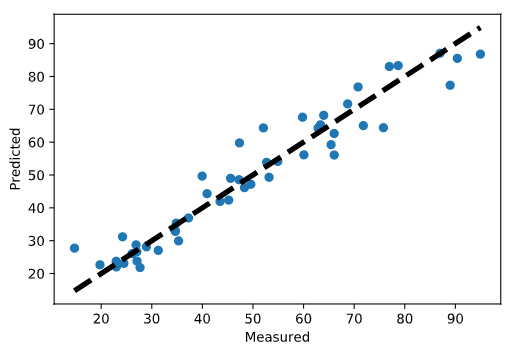
\includegraphics[width=0.7\textwidth]{results/lin-reg-measured-vs-pred.png}
\end{center}
\end{answerbox}



\end{subquestion}



%
%
\begin{subquestion}{(3 points) Instead of using sklearn, implement the closed-form solution for fitting a linear regression model yourself using numpy array operations.  
Report your code in the answer box.
It should only take a few lines (i.e. <5).\\ 
\hint{Only report the relevant lines for estimating $\mathbf{w}$ e.g. we do not need to see the data loading code. You can write the code in the answer box directly or paste in an image of it. }
}


\begin{answerbox}{20em}
To estimate the parameters we use the formula $\beta = (X^{T}X)^{-1}X^{T}y$
\begin{verbatim}
w = np.linalg.inv(X.transpose().dot(X)).dot(X.transpose()).dot(y)
\end{verbatim}
\end{answerbox}



\end{subquestion}



%
%
\begin{subquestion}{(3 points) Mean Squared Error (MSE) is a common metric used for evaluating the performance of regression models. 
Write out the expression for MSE and list one of its limitations. \\
\hint{For notation, you can use $y$ for the ground truth quantity and $\hat{y}$ (\texttt{\$\textbackslash{}hat\{y\}\$} in latex) in place of the model prediction.}
}


\begin{answerbox}{10em}
$$MSE = \frac{1}{n}\sum_{t=1}^{n}(y_{i} - \hat{y_{i}})^2$$

Mean Squared Error is prone to outliers. When we calculate our mean there is a chance that it might be a very large value due to one large outlier. This can produce high errors.
\end{answerbox}



\end{subquestion}


 
%
%
\begin{subquestion}{(3 points) Our next step will be to evaluate the performance of the fitted models using Mean Squared Error (MSE). 
Report the MSE of the data in \texttt{regression\_part1.csv} for your prediction of \texttt{exam\_score}.
You should report the MSE for the linear model fitted using sklearn and the model resulting from your closed-form solution. 
Comment on any differences in their performance. 
}


\begin{answerbox}{10em}
MSE of the sklearn model is $30.9854726145413$ , and of the closed form solution model is $30.98547261454129$. As we can see the difference is of the order $10^{-14}$ and hence completely negligible.
\end{answerbox}



\end{subquestion}




%
%
\begin{subquestion}{(4 points) Assume that the optimal value of $w_0$ is $20$, it is not but let's assume so for now. 
Create a plot where you vary $w_1$ from $-2$ to $+2$ on the horizontal axis, and report the Mean Squared Error on the vertical axis for each setting of $\mathbf{w} = [w_0, w_1]$ across the dataset. 
Describe the resulting plot. Where is its minimum? Is this value to be expected?\\ 
\hint{You can try 100 values of $w_1$ i.e. \texttt{w1 = np.linspace(-2,2, 100)}.}
}


\begin{answerbox}{35em}
\begin{center}
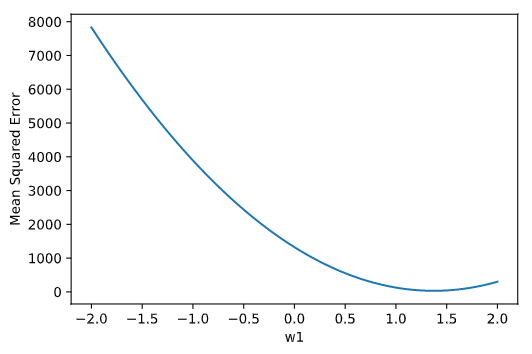
\includegraphics[width=0.7\textwidth]{results/mse-vs-ws.png}
\end{center}
The plot is in the shape of an half-parabola, if we extend the x-axis we will see the full parabolic graph. The minima of the plot is at $w1 = 1.3535353535353538$. This can be explained by its closeness to the actual value of $\beta = 1.44114091$, which we found when we fitted our model. The slight discrepancy can be explained by choosing an non optimal value for $w0$ instead of $17.89768026$.

\end{answerbox}



\end{subquestion}


 
\end{question}





%%%%%%%%%%%%%%%%%%%%%%%%%%%%%%%%%%%%%%%%%%%%%%%%%%%%%%%%%%%%%%%%%%%%%%%%%%%%%%
%============================================================================%
%%%%%%%%%%%%%%%%%%%%%%%%%%%%%%%%%%%%%%%%%%%%%%%%%%%%%%%%%%%%%%%%%%%%%%%%%%%%%%
\clearpage



\begin{question}{(18 total points) Nonlinear Regression}

\questiontext{In this question we will tackle regression using basis functions.}




%
%
\begin{subquestion}{(5 points) Fit four different polynomial regression models to the data  by varying the degree of polynomial features used i.e. $M = 1$ to $4$.
For example, $M=3$ means that $\boldsymbol{\phi}(x_i) = [1, x_i, x_i^2, x_i^3]$.
Plot the resulting models on the same plot and also include the input data.\\
\hint{
 You can again use the sklearn implementation of \href{https://scikit-learn.org/0.19/modules/generated/sklearn.linear_model.LinearRegression.html}{Linear Regression} and you can also use \href{https://scikit-learn.org/0.19/modules/generated/sklearn.preprocessing.PolynomialFeatures.html}{PolynomialFeatures} to generate the polynomial features. Again, set \texttt{fit\_intercept = False}.}
}


\begin{answerbox}{35em}
\begin{center}
    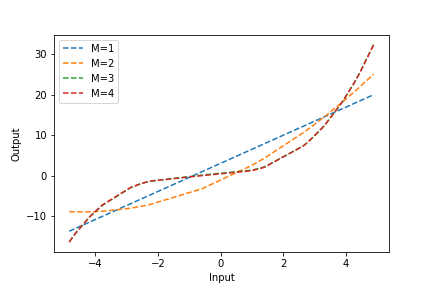
\includegraphics[width=0.7\textwidth]{results/input-vs-output-nonlinear.png}
\end{center}
\end{answerbox}



\end{subquestion}


%
%
\begin{subquestion}{(3 points) Create a bar plot where you display the Mean Squared Error of each of the four different polynomial regression models from the previous question.}


\begin{answerbox}{35em}
Your Answer Here
\end{answerbox}



\end{subquestion}


%
%
\begin{subquestion}{(4 points) Comment on the fit and Mean Squared Error values of the $M=3$ and $M=4$ polynomial regression models. 
Do they result in the same or different performance? 
Based on these results, which model would you choose?}


\begin{answerbox}{15em}
Your Answer Here
\end{answerbox}



\end{subquestion}



%
%
\begin{subquestion}{(6 points) Instead of using polynomial basis functions, in this final part we will use another type of basis function - radial basis functions (RBF). 
Specifically, we will define $\boldsymbol{\phi}(x_i) = [1, rbf(x_i; c_1, \alpha), rbf(x_i; c_2, \alpha), rbf(x_i; c_3, \alpha), rbf(x_i; c_4, \alpha)]$, where $rbf(x; c, \alpha) =  \exp(-0.5(x-c)^2 / \alpha^2)$ is an RBF kernel with center $c$ and width $\alpha$. Note that in this example, we are using the same width $\alpha$ for each RBF, but different centers for each.\\ 
Let $c_1=-4.0$, $c_2=-2.0$, $c_3=2.0$, and $c_4=4.0$ and plot the resulting nonlinear predictions using the \texttt{regression\_part2.csv} dataset for $\alpha \in \{0.2, 100, 1000\}$. 
You can plot all three results on the same figure.
Comment on the impact of larger or smaller values of $\alpha$.
}


\begin{answerbox}{35em}
Your Answer Here
\end{answerbox}



\end{subquestion}



\end{question}






%%%%%%%%%%%%%%%%%%%%%%%%%%%%%%%%%%%%%%%%%%%%%%%%%%%%%%%%%%%%%%%%%%%%%%%%%%%%%%
%============================================================================%
%%%%%%%%%%%%%%%%%%%%%%%%%%%%%%%%%%%%%%%%%%%%%%%%%%%%%%%%%%%%%%%%%%%%%%%%%%%%%%
\clearpage


\begin{question}{(26 total points) Decision Trees}

\questiontext{In this question we will train a classifier to predict if a person is smiling or not.}




%
%
\begin{subquestion}{(4 points) Load the data, taking care to separate the target binary class label we want to predict, \texttt{smiling}, from the input attributes. 
Summarise the main properties of both the training and test splits. 
}


\begin{answerbox}{12em}
Your Answer Here
\end{answerbox}



\end{subquestion}


%
%
\begin{subquestion}{(4 points) Even though the input attributes are high dimensional, they actually consist of a set of 2D coordinates representing points on the faces of each person in the dataset. 
Create a scatter plot of the average location for each 2D coordinate. One for (i) smiling and (ii) one not smiling faces. 
For instance, in the case of smiling faces, you would average each of the rows where \texttt{smiling = 1}. 
You can plot both on the same figure, but use different colors for each of the two cases. 
Comment on any difference you notice between the two sets of points. \\
\hint{Your plot should contain two faces.}
}


\begin{answerbox}{35em}
Your Answer Here
\end{answerbox}



\end{subquestion}


%
%
\begin{subquestion}{(2 points) 
There are different measures that can be used in decision trees when evaluating the quality of a split. 
What measure of purity at a node does the \href{https://scikit-learn.org/0.19/modules/generated/sklearn.tree.DecisionTreeClassifier.html}{DecisionTreeClassifier} in sklearn use for classification by default? 
What is the advantage, if any, of using this measure compared to entropy? 
}


\begin{answerbox}{10em}
Your Answer Here
\end{answerbox}



\end{subquestion}


%
%
\begin{subquestion}{(3 points) 
One of the hyper-parameters of a decision tree classifier is the maximum depth of the tree. 
What impact does smaller or larger values of this parameter have? Give one potential problem for small values and two for large values. 
}


\begin{answerbox}{10em}
Your Answer Here
\end{answerbox}



\end{subquestion}


%
%
\begin{subquestion}{(6 points) 
Train three different decision tree classifiers with a maximum depth of 2, 8, and 20 respectively.
Report the maximum depth, the training accuracy (in \%), and the test accuracy (in \%) for each of the three trees.
Comment on which model is best and why it is best. \\
\hint{Set \texttt{random\_state = 2001} and use the \texttt{predict()} method of the \href{https://scikit-learn.org/0.19/modules/generated/sklearn.tree.DecisionTreeClassifier.html}{DecisionTreeClassifier} so that you do not need to set a threshold on the output predictions.
You can set the maximum depth of the decision tree using the \texttt{max\_depth} hyper-parameter.}
}


\begin{answerbox}{20em}
Your Answer Here
\end{answerbox}



\end{subquestion}


%
%
\begin{subquestion}{(5 points) 
Report the names of the top three most important attributes, in order of importance, according to the Gini importance from \href{https://scikit-learn.org/0.19/modules/generated/sklearn.tree.DecisionTreeClassifier.html}{DecisionTreeClassifier}. 
Does the one with the highest importance make sense in the context of this classification task? \\
\hint{Use the trained model with \texttt{max\_depth = 8} and again set  \texttt{random\_state = 2001}.}
}


\begin{answerbox}{10em}
Your Answer Here
\end{answerbox}



\end{subquestion}



%
%
\begin{subquestion}{(2 points) 
Are there any limitations of the current choice of input attributes used i.e. 2D point locations? If so, name one. 
}


\begin{answerbox}{10em}
Your Answer Here
\end{answerbox}



\end{subquestion}


\end{question}




%%%%%%%%%%%%%%%%%%%%%%%%%%%%%%%%%%%%%%%%%%%%%%%%%%%%%%%%%%%%%%%%%%%%%%%%%%%%%%
%============================================================================%
%%%%%%%%%%%%%%%%%%%%%%%%%%%%%%%%%%%%%%%%%%%%%%%%%%%%%%%%%%%%%%%%%%%%%%%%%%%%%%
\clearpage


\begin{question}{(14 total points) Evaluating Binary Classifiers}

\questiontext{In this question we will perform performance evaluation of binary classifiers.}




%
%
\begin{subquestion}{(4 points) Report the classification accuracy (in \%) for each of the four different models using the \texttt{gt} attribute as the ground truth class labels. 
Use a threshold of $>= 0.5$ to convert the continuous classifier outputs into binary predictions. 
Which model is the best according to this metric?
What, if any, are the limitations of the above method for computing accuracy and how would you improve it without changing the metric used?
}


\begin{answerbox}{15em}
Your Answer Here
\end{answerbox}



\end{subquestion}



%
%
\begin{subquestion}{(4 points) Instead of using classification accuracy, report the Area Under the ROC Curve (AUC) for each model. 
Does the model with the best AUC also have the best accuracy? If not, why not?\\
\hint{You can use the  \href{https://scikit-learn.org/0.19/modules/generated/sklearn.metrics.roc\_auc\_score.html}{roc\_auc\_score} function from sklearn.}
}


\begin{answerbox}{15em}
Your Answer Here
\end{answerbox}



\end{subquestion}



%
%
\begin{subquestion}{(6 points) Plot ROC curves for each of the four models on the same plot.
Comment on the ROC curve for \texttt{alg\_3}?
Is there anything that can be done to improve the performance of \texttt{alg\_3} without having to retrain the model?\\
\hint{You can use the \href{https://scikit-learn.org/0.19/modules/generated/sklearn.metrics.roc\_curve.html}{roc\_curve} function from sklearn.}
}


\begin{answerbox}{35em}
Your Answer Here
\end{answerbox}



\end{subquestion}

\end{question}







\end{document}